\section{Full Experimental Results}
\label{sec:experiment_details}

\subsection{BERT}
\label{subsec:bert_details}

We train BERT-large following the training procedure and hyperparameters of the
reference MLPerf 1.1 implementation.
In particular, we use the LAMB optimizer with learning rate 3.75e-3, with batch
size 448, trained for at most 7100 steps.
The training is stopped once the validation accuracy (for masked language
modeling) reaches the target 72.0\%, and the wall-clock run-time is measured.
We train with FP16 precision using Apex AMP (with O2 optimization level).

We compare our results with the reported training speed from Nvidia that was
submitted to MLPerf 1.1 (\cref{table:bert_speed}).

We use the same train / validation data split provided by MLPerf 1.1 reference
implementation.
In particular, we evaluate on the same 10000 validation examples as the
baseline from Nvidia.

We train the model on 8$\times$A100-80GB GPUs. Each training run takes between 16
and 19 minutes, and we average the results of 10 runs.

\subsection{GPT-2}
\label{subsec:gpt_details}

We use the standard implementations of
GPT-2~\citep{radford2019language} from Huggingface \texttt{transformers} library and from Nvidia's Megatron-LM repo.
We follow the training recipe of the Megatron-LM repo.

We use an effective batch size of 512, and use gradient accumulation to fit into
available GPU memory.
We use the AdamW optimizer, with learning rate 6e-4 for GPT-2 small and 1.5e-4
for GPT-2 medium, and weight decay of 0.1.
All models are trained with the same hyperparameters for 400K steps.
We run all implementations with mixed-precision training (PyTorch AMP).

We use the Openwebtext dataset, with the GPT-2 BPE tokenizer. We randomly select
0.5\% of the dataset as the validation set, with the rest being used as training
set.
This random selection of validation set is done once, and all models are evaluated
on the same validation set.

We train the model on 8$\times$A100-40GB GPUs, and we measure the wall-clock training
time.
Training GPT-2 small takes between 2.7-9.5 days, and training GPT-2 medium takes
between 6.9-21.0 days (\cref{table:gpt_finetune}).

In~\cref{fig:gpt2_training_curve}, we plot of the validation perplexity throughout training of GPT-2 small/medium,
using either HuggingFace implementation or our \sysname implementation.
We see that \sysname behaves the same as the baseline implementation
and the validation perplexity curves of the two implementations almost lie on
top of each other.

\begin{figure}[ht]
  \centering
  \includegraphics[width=0.7\textwidth]{figs/gpt2_flashattn_training.pdf}
  \caption{\label{fig:gpt2_training_curve}Validation perplexity of GPT-2
    small/medium using two implementations.
    We confirm that \sysname yields the same validation curves as the baseline
    implementation from HuggingFace.}
\end{figure}

\iftoggle{icmlworkshop}{
\subsection{Faster Transformer with \sysname on Long-range Arena}
We compare vanilla Transformer (with either standard implementation or \sysname)
on the long-range arena (LRA~\citep{tay2020long}) benchmark.
We measure accuracy, throughput, and training time of all models.
Each task has a different sequence length varying between 1024 and 4096.
We follow the implementation and experimental setting
in~\citet{tay2020long}and~\citet{xiong2021nystromformer}.\footnote{LRA accuracy
  results are known to be highly dependent on the tuning
  procedure~\citep{xiong2021nystromformer}.
  Our reproduced baselines perform better than as reported in the original
  comparison~\citep{tay2020long}.}
\cref{table:lra} shows that \sysname achieves up 2.4$\times$
speed-up compared to standard attention.
Block-sparse \sysname is faster than all of the approximate attention methods that we have
tested.

\begin{table}[h]
\captionsetup{font=small}
  \vspace{-1em}
    \caption{The performance of standard attention, \sysname, block-sparse
      \sysname, and approximate attention baselines on the Long-Range-Arena benchmarks.}
	\centering
	\small
  \iftoggle{arxiv}{}{
    \resizebox{0.9\linewidth}{!}
  }
  {
	\begin{tabular}{c|ccccc|c|c}
  Models & ListOps & Text & Retrieval & Image & Pathfinder & Avg & Speedup \\
	\hline
	Transformer & 36.0 & 63.6 & 81.6 & 42.3 & 72.7 & 59.3 & - \\
  \sysname & 37.6 & 63.9 & 81.4 & 43.5 & 72.7 & 59.8 & 2.4$\times$ \\
  Block-sparse \sysname & 37.0 & 63.0 & 81.3 & 43.6 & 73.3 & 59.6 & \textbf{2.8$\times$} \\
	\cline{1-8}
	\hline
  Linformer~\citep{wang2020linformer} & 35.6 & 55.9 & 77.7 & 37.8 & 67.6 & 54.9 & 2.5$\times$ \\
  Linear Attention~\citep{katharopoulos2020transformers} & 38.8 & 63.2 & 80.7 & 42.6 & 72.5 & 59.6 & 2.3$\times$ \\
  Performer~\citep{choromanski2020rethinking} & 36.8 & 63.6 & 82.2 & 42.1 & 69.9 & 58.9 & 1.8$\times$ \\
  Local Attention~\citep{tay2020long} & 36.1 & 60.2 & 76.7 & 40.6 & 66.6 & 56.0 & 1.7$\times$ \\
  Reformer~\citep{kitaev2020reformer} & 36.5 & 63.8 & 78.5 & 39.6 & 69.4 & 57.6 & 1.3$\times$  \\
  Smyrf~\citep{daras2020smyrf} & 36.1 & 64.1 & 79.0 & 39.6 & 70.5 & 57.9 & 1.7$\times$ \\
	\end{tabular}
  }
	\label{table:lra}
	\vspace{-1em}
\end{table}

\subsection{Better Models with Longer Sequences}
\label{ssec:exp_long_sequences}


\paragraph{Language Modeling with Long Context.}
The runtime and memory-efficiency of \sysname allow us to increase the context length of
GPT-2 by 4$\times$ while still running faster than the optimized
implementation from Megatron-LM.
\cref{table:gpt2_long_context} shows that that GPT-2 with \sysname and
context length 4K is still 30\% faster than GPT-2 from Megatron with context
length 1K, while achieving 0.7 better perplexity.

\begin{table}[h]
\vspace{-3mm}
  \captionsetup{font=small}
  \small
  \centering
  \caption{\label{table:gpt2_long_context}GPT-2 small with \sysname, with 4$\times$ larger context
    length compared to Megatron-LM, is still 30\% faster while achieving 0.7
    better perplexity. Training time on 8$\times$A100 GPUs is reported.}
  \setlength{\tabcolsep}{5pt}
  \vspace{1em}
  \iftoggle{arxiv}{}{
      \resizebox{0.8\linewidth}{!}
  }
  {
    \begin{tabular}{@{}c|ccc@{}}
      Model implementations & Context length &\multicolumn{1}{c}{OpenWebText (ppl)}&\multicolumn{1}{c}{Training time (speedup)} \\
    \hline
      GPT-2 small - Megatron-LM & 1k & 18.2 & 4.7 days (1.0$\times$) \\
      GPT-2 small - \sysname & 1k & 18.2 & \textbf{2.7 days (1.7$\times$)} \\
      GPT-2 small - \sysname & 2k & 17.6 & 3.0 days (1.6$\times$) \\
      GPT-2 small - \sysname & 4k & \textbf{17.5} & 3.6 days (1.3$\times$) \\
    \end{tabular}
  }
  \vspace{-3mm}
\end{table}
}{}

\paragraph{Long Document Classification.}
\iftoggle{icmlworkshop}{
Training Transformers with longer sequences with \sysname improves performance on the MIMIC-III~\citep{johnson2016mimic} and ECtHR~\citep{chalkidis-etal-2019-neural, chalkidis-et-al-2021-ecthr} datasets.
MIMIC-III contains intensive care unit patient discharge summaries, each annotated with multiple labels.
ECtHR contains legal cases from the European Court of Human Rights, each of which is mapped to articles of the Convention of Human Rights that were allegedly violaged.
Both of these datasets contain very long text documents; the average number of tokens in MIMIC is 2,395 tokens, and the longest document contains 14,562 tokens, while the average and longest numbers in ECtHR are 2,197 and 49,392, respectively.
We evaluate lift from increasing the sequence length of a pretrained RoBERTa model~\citep{liu2019roberta} (we repeat the positional embeddings, as in~\citet{beltagy2020longformer}).

Table~\ref{tab:mimic} shows that sequence length 16K outperforms length 512 by 4.3 points on MIMIC, and that  length 8K outperforms length 512 by 8.5 points on ECtHR.
The discrepancies may be due to subtle distribution shifts: MIMIC-III contains specialized medical text and thus may be more susceptible to a distribution shift in the document length, whereas ECtHR contains general language.

\vspace{-1em}
\begin{table}[h]
    \centering
    \begin{minipage}{2.5in}
    \small
\captionsetup{font=small}
\caption{Long Document performance (micro $F_1$) at different sequence lengths using \sysname.}
\resizebox{1.05\linewidth}{!}
{
\begin{tabular}{@{}r|ccccccccc@{}}
 & 512 & 1024 & 2048 & 4096 & 8192 & 16384 \\
\hline
MIMIC-III~\citep{johnson2016mimic} & 52.8 & 50.7 & 51.7 & 54.6 & 56.4 & \textbf{57.1} \\
ECtHR~\citep{chalkidis-etal-2019-neural} & 72.2 & 74.3 & 77.1 & 78.6 & \textbf{80.7} & 79.2 \\
\end{tabular}
}
\label{tab:mimic}

    \end{minipage}
    \begin{minipage}{0.20in}
    ~
    \end{minipage}
    \begin{minipage}{2.5in}
    \captionsetup{font=small}
    \caption{We report the first Transformer model that can achieve non-random performance on Path-X and Path-256.}
	\centering
	\small
  \resizebox{0.95\linewidth}{!}
  {
	\begin{tabular}{c|cc}
    {\bf Model}  & Path-X & Path-256 \\
	\hline
	Transformer& \xmark & \xmark \\
	Linformer~\citep{wang2020linformer}& \xmark & \xmark \\
	Linear Attention~\citep{katharopoulos2020transformers}& \xmark & \xmark \\
	Performer~\citep{choromanski2020rethinking}& \xmark & \xmark \\
	Local Attention~\citep{tay2020long} & \xmark & \xmark \\
	Reformer~\citep{kitaev2020reformer}& \xmark & \xmark \\
	SMYRF~\citep{daras2020smyrf}& \xmark & \xmark \\
	
    \hline
    \sysname & \textbf{61.4} & \xmark \\
    Block-sparse \sysname & 56.0 & \textbf{63.1} \\
	
	\end{tabular}
  }
	\label{table:pathx}

    \end{minipage}
\end{table}
\vspace{-1em}
}{}

For MIMIC-III and ECtHR, we follow the hyperparameters of~\citet{dai2022revisiting}.

\subsection{LRA details}
\label{subsec:lra_details}

We follow the hyperparameters from the Long-range arena
paper~\citep{tay2020long}, the Long-range arena repo
(\url{https://github.com/google-research/long-range-arena}), and the
Nystr{\"o}mformer reproduction~\citep{xiong2021nystromformer}.
To be generous to the baseline methods, if we are unable to reproduce the
performance of any baseline for any of the five tasks, we report the better
performance from~\citet{tay2020long} or~\citet{xiong2021nystromformer} for that
baseline on that task.

After hyperparameter tuning, almost all of the attention methods achieve similar
accuracy on all of the five LRA tasks.

We run all methods with mixed-precision training, except for Performer (not
stable with mixed precision) and Local Attention (implementation does not
support FP16).

To calculate the overall wallclock-time speedup, we take the geometric mean of
the wallclock-time speedup of each of the five tasks.

\paragraph{Path-X}
For Path-X and Path-256, we follow the hyperparameters from the PathFinder-32 experiments from the long-range arena paper\citep{tay2020long}.
For both, we first pretrain a model on Path-64.
We take the checkpoint after 200 epochs, upsample its positional embedding (we duplicate the positional embeddings gridwise in space), and fine-tune it on the downstream task for 200 epochs with one epoch of linear warmup, and cosine decay of the learning rate.
For Path-X, we take the best performing checkpoint (according to val accuracy), and additionally fine-tune it for 200 epochs with the same warmup and learning rate (this adds roughly 4 points of accuracy to \sysname for Path-X, but the model starts overfitting afterwards).

\iftoggle{icmlworkshop}{
\subsection{Benchmarking Attention}
\label{sec:benchmark}






\begin{figure}
\centering
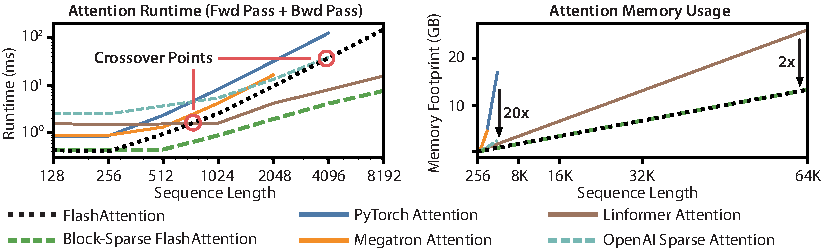
\includegraphics[width=5.5in]{figs/attention_benchmarks.pdf}
\iftoggle{arxiv}{}{
\vspace{-1em}
}
\caption{\textbf{Left:} runtime of forward pass + backward pass. \textbf{Right:} attention memory usage.}
\label{fig:benchmark}
\iftoggle{arxiv}{}{
\vspace{-1.0em}
}
\end{figure}



We vary sequence length and measure runtime and memory usage of \sysname and block-sparse \sysname against various attention baselines on one A100 GPU with 40 GB HBM, with dropout and a padding mask.
We compare against reference implementations for exact attention, approximate attention, and sparse attention.
We report a subset of baselines in the main body; Appendix~\ref{sec:experiment_details} contains more baselines and full details.




\paragraph{Runtime.}
Figure~\ref{fig:benchmark} (left) reports the runtime in milliseconds of the forward + backward pass of \sysname and block-sparse \sysname compared to the baselines in exact, approximate, and sparse attention (exact numbers in Appendix~\ref{sec:experiment_details}).
Runtime grows quadratically with sequence length, but \sysname runs significantly faster than \textbf{exact attention} baselines, up to 3$\times$ faster than the PyTorch implementation.
The runtimes of many approximate/sparse attention mechanisms grow linearly with sequence length, but \sysname still runs faster than approximate and sparse attention for short sequences due to fewer memory accesses.
The \textbf{approximate attention} runtimes begin to cross over with \sysname at sequences between 512 and 1024.
On the other hand, block-sparse \sysname is faster than all implementations of exact, sparse, and approximate attention that we know of, across all sequence lengths.

\paragraph{Memory Footprint.}
Figure~\ref{fig:benchmark} (right) shows the memory footprint of \sysname and block-sparse \sysname compared to various exact, approximate, and sparse attention baselines.
\sysname and block-sparse \sysname have the same memory footprint, which grows linearly with sequence length.
\sysname is up to 20$\times$ more memory efficient than \textbf{exact attention} baselines, and is more memory-efficient than the \textbf{approximate attention} baselines.
All other algorithms except for Linformer run out of memory on an A100 GPU before 64K, and \sysname is still 2$\times$ more efficient than Linformer.
}{}

\subsection{Comparison with Apex FMHA}
\label{supp:fmha}

We compare our method/implementation with Apex FMHA
(\url{https://github.com/NVIDIA/apex/tree/master/apex/contrib/csrc/fmha}).

When we started this project, Apex FMHA was the fastest implementation of
attention (that we knew of), tailored for short sequences of length at most 512.
In fact, almost all MLPerf submissions for BERT training benchmark running on
Nvidia GPUs use FMHA for their model code, as of MLPerf
1.1~\citep{mattson2020mlperf}.
Since FMHA targets BERT models, it only supports head
dimension 64, and only runs on A100 GPUs.
FMHA fuses the attention computation
$\mathrm{dropout}(\softmax(\textsc{mask}(\vQ \vK^\top))) \vV$ into one CUDA kernel.
In the forward pass, it stores the attention matrix
$\softmax(\textsc{mask}(\vQ \vK^T))$ to HBM to be used in gradient computation.
As a result, it does not offer substantial memory saving (though for shorter
sequences memory footprint is often not a primary concern).

We use FMHA code as a starting point, and apply two well-established techniques
(tiling and recomputation) to deal with long sequences and to save memory as
mentioned in~\cref{sec:algo}.
As a result, we can support much longer sequences (e.g., up to length 64K).
We also support more head dimensions (16, 32, 64, 128) and broader GPU types
(all Turing and Ampere GPUs at the time of writing).

In~\cref{tab:fmha_comparison}, we compare the performance of \sysname and Apex FMHA for short sequences
(as FMHA only supports sequence length at most 512).
Generally \sysname is slightly faster than FMHA in the forward pass and slightly
slower than FMHA in the backward pass.
This is because we do not store the attention matrix in the forward pass and
recompute it in the backward pass.
Compared to FMHA, the overall runtime of \sysname is about 4\% slower for sequence length 128, 8\%
faster for sequence length 256, and 5\% faster for sequence length 512.
\begin{table}
\centering
\small
\captionsetup{font=small}
\caption{Runtime (ms) of \sysname compared to FMHA by sequence length, with
  masking and dropout, measured on an A100-SXM4-40GB GPU. Batch size 64, 16
  heads, head dimension 64 (i.e., BERT-large size).}
\begin{tabular}{@{}r|ccc@{}}
\toprule
\textbf{Attention Method} & 128 & 256 & 512 \\
\hline
\textbf{Apex FMHA forward} & 0.10 & 0.29 & 1.14 \\
\textbf{\sysname forward} & \textbf{0.08} & \textbf{0.22} & \textbf{0.81} \\
\hline
\textbf{Apex FMHA backward} & \textbf{0.17} & \textbf{0.52} & \textbf{1.81} \\
\textbf{\sysname backward} & 0.20 & 0.53 & 2.00 \\
\hline
\textbf{Apex FMHA forward + backward} & \textbf{0.27} & 0.81 & 2.95 \\
\textbf{\sysname forward + backward} & 0.28 & \textbf{0.75} & \textbf{2.81} \\
\hline
\bottomrule
\end{tabular}
\label{tab:fmha_comparison}
\end{table}

\subsection{Speedup On Different Hardware and Configurations}
\label{supp:hardware}

Speedup varies between different types of GPU types and generations depending on HBM bandwidth and SRAM size.
In this section, we profile \sysname speedup on different GPUs and configurations.

\begin{figure}[h!]
  \centering
  \includegraphics[width=5.5in]{figs/flashattn_speedup.jpg}
  \caption{Speedup over standard PyTorch attention at different sequence lengths, on A100.}
  \label{fig:A100_speedup}
\end{figure}

\paragraph{A100}
Figure~\ref{fig:A100_speedup} shows speedup on an A100 GPU with batch size 8, head dimension 64, and 12 attention heads, across different sequence lengths.
We generally see 2-4$\times$ speedup, and we see more speedup when using dropout and masking due to kernel fusion.

\begin{figure}[h!]
  \centering
  \includegraphics[width=5.5in]{figs/flashattn_speedup_a100_d128.jpg}
  \caption{Speedup over standard PyTorch attention at different sequence lengths, on A100, with head dimension 128.}
  \label{fig:A100_speedup_128_dim}
\end{figure}
\paragraph{A100, Head Dimension 128}
Speedup also changes when we increase the head dimension.
Each block requires more memory, so we need to use smaller block sizes to fit into SRAM.
Figure~\ref{fig:A100_speedup_128_dim} shows speedup with head dimension 128 on an A100 (batch size 16, 12 heads).
We see less speedup overall---but we can still see significant speedup (up to 3$\times$) with a causal mask, where half the blocks are masked out.

\begin{figure}[h!]
  \centering
  \includegraphics[width=5.5in]{figs/flashattn_speedup_3090.jpg}
  \caption{Speedup over standard PyTorch attention at different sequence lengths, on RTX 3090.}
  \label{fig:rtx3090_speedup}
\end{figure}

\paragraph{RTX 3090}
Figure~\ref{fig:rtx3090_speedup} shows speedup on an RTX 3090 GPU.
Here, we use batch size 12 with 12 attention heads.
We observe slightly higher speedups on the RTX 3090 (between 2.5-4.5$\times$), since the memory bandwidth on an RTX 3090 is lower than on an A100 (roughly 900 GB/s vs. 1.5 TB/s).

\begin{figure}[h!]
  \centering
  \includegraphics[width=5.5in]{figs/flashattn_speedup_t4.jpg}
  \includegraphics[width=5.5in]{figs/flashattn_speedup_t4_fwd.jpg}
  \caption{Speedup over standard PyTorch attention at different sequence lengths, on T4. \textbf{Top:} Combined forward pass + backward pass. \textbf{Bottom:} Forward pass only.}
  \label{fig:t4_speedup}
\end{figure}

\paragraph{T4}
Figure~\ref{fig:t4_speedup} shows speedup on a T4 GPU. T4 SRAM is smaller than A100, so we need to make the block sizes smaller in \sysname.
As a result, we observe less speedup on T4, which matches the IO complexity analysis in Section~\ref{sec:theory}.
T4 GPUs are commonly used for inference, so we also report speedup on the forward pass only.

\subsection{Full Benchmarking Results}
\label{supp:benchmarking}

We report the full benchmarking results and experimental details on A100.

\paragraph{Baselines}
We compare against reference implementations for exact attention from PyTorch/HuggingFace and Megatron, approximate attention, and sparse attention.
For approximate attention, we compare against reference implementations of Reformer~\citep{kitaev2020reformer}, Local Attention~\citep{rae-razavi-2020-transformers}, Linformer Attention~\citep{wang2020linformer}, Smyrf~\citep{daras2020smyrf}, and LongShortFormer (LSFormer)~\citep{zhu2021long}.
For sparse attention, we compare against reference implementations of Block-Sparse Attention form OpenAI~\citep{child2019generating}, Longformer\citep{beltagy2020longformer}, and BigBird Attention~\citep{zaheer2020bigbird}.
For the approximate and sparse attention, we use a compression ratio of 1/8, or a compressed sequence length of 256, whichever is smaller.

\paragraph{Setup}
We measure runtime and memory usage of the attention computation with 8 heads of dimension 64, and batch size 16 on a machine with one A100 GPU with 40 GB of GPU HBM.
We vary sequence length in our experiments.
We compute attention on random vectors for $\vQ$, $\vK$, and $\vV$ (we do not measure the projection from the hidden layer).
For dropout, we use dropout 0.1; for masking, we use a padding mask with uniformly-random mask lengths between the total sequence length and the total sequence length minus 20.
To measure runtime, we take the average of 100 measurements of the attention call.
We only measure memory footprint once, since it does not vary between runs.

We report timing results on the forward pass, backward pass, and combined forward + backward pass.
We measure each method with and without dropout, masking, or both---except for Block Sparse, Longformer, and BigBird.
These methods did not successfully run the backward pass with masking due to a bug in external libraries, so we measured them without masking to be generous.
We use FP16 for all measurements, except for Local Attention, whose
implementation only supports FP32.

For each baseline, we increase sequence length until it runs out of memory on the GPU, except for the following exceptions:
The Megatron implementation does not support sequence lengths longer than 2048.
Block-Sparse (OpenAI) does not support sequence lengths longer than 4096.
Longformer and BigBird do not support sequence lengths longer than 8092.

We measure memory usage on the combined forward + backward pass, without dropout or masking.

\paragraph{Results}
\cref{tab:benchmark_summary} summarizes all the experimental configurations and contains pointers to the results tables.

\begin{table}
    \centering
    \caption{Pointers to results tables.}
    \label{tab:benchmark_summary}
    \begin{tabular}{ccc|c}
    \toprule
        \textbf{Dropout} & \textbf{Masking} & \textbf{Pass} & \textbf{Table} \\ \hline
        Yes & Yes & Forward & \cref{tab:dropout_masking_forward_pass} \\
        Yes & Yes & Backward & \cref{tab:dropout_masking_backward_pass} \\
        Yes & Yes & Combined & \cref{tab:dropout_masking_combined} \\
        No & Yes & Forward  & \cref{tab:masking_forward_pass} \\
        No & Yes & Backward & \cref{tab:masking_backward_pass} \\
        No & Yes & Combined & \cref{tab:masking_combined} \\
        Yes & No & Forward  & \cref{tab:dropout_forward_pass} \\
        Yes & No & Backward & \cref{tab:dropout_backward_pass} \\
        Yes & No & Combined & \cref{tab:dropout_combined} \\
        No & No & Forward  & \cref{tab:forward_pass} \\
        No & No & Backward & \cref{tab:backward_pass} \\
        No & No & Combined & \cref{tab:combined} \\
        No & No & Memory Usage (Combined) & \cref{tab:memory} \\
        \toprule
    \end{tabular}
\end{table}

\begin{table}
\centering
\scriptsize
\captionsetup{font=small}
\caption{Forward pass runtime (ms) of various exact/approximate/sparse attention mechanisms by sequence length, \textbf{with dropout and masking}. Best in \textbf{bold}, second best \underline{underlined}.}
\begin{tabular}{@{}r|cccccccccc@{}}
\toprule
\textbf{Attention Method} & 128 & 256 & 512 & 1024 & 2048 & 4096 & 8192 & 16384 & 32768 & 65536 \\
\hline
\textbf{PyTorch Attention} & 0.36 & 0.34 & 0.78 & 2.54 & 9.33 & 36.33 & - & - & - & - \\
\textbf{Megatron} & 0.40 & 0.40 & 1.10 & 3.65 & 16.19 & - & - & - & - & - \\
\hline
\textbf{Reformer} & 2.03 & 3.15 & 5.67 & 11.02 & 22.59 & 46.14 & 97.38 & 212.13 & - & - \\
\textbf{Local Attention} & 0.83 & 0.86 & 1.01 & 2.20 & 7.13 & 14.32 & 28.60 & 57.79 & 117.67 & - \\
\textbf{Linformer} & 0.67 & 0.52 & 0.69 & \underline{0.71} & \underline{1.65} & \underline{3.18} & \underline{6.15} & \underline{12.16} & \underline{24.17} & \underline{52.39} \\
\textbf{Smyrf} & 2.27 & 2.34 & 3.91 & 7.44 & 14.71 & 29.22 & 58.27 & 116.41 & - & - \\
\textbf{LSformer} & 1.18 & 1.27 & 1.34 & 3.38 & 11.40 & 22.55 & 44.95 & 89.76 & 179.66 & - \\
\hline
\textbf{Block Sparse} & 1.12 & 1.11 & 2.13 & 2.77 & 6.95 & 20.91 & - & - & - & - \\
\textbf{Longformer} & 1.22 & 1.14 & 1.08 & 1.95 & 5.72 & 12.98 & - & - & - & - \\
\textbf{BigBird} & 1.13 & 1.12 & 1.12 & 1.77 & 6.03 & 13.68 & - & - & - & - \\
\hline
\textbf{\sysname} & \textbf{0.04} & \underline{0.06} & \underline{0.21} & 0.82 & 2.85 & 10.41 & 41.74 & 167.19 & 670.76 & 2682.35 \\
\textbf{Block-Sparse \sysname} & \underline{0.06} & \textbf{0.06} & \textbf{0.06} & \textbf{0.12} & \textbf{0.44} & \textbf{0.86} & \textbf{1.70} & \textbf{3.29} & \textbf{6.55} & \textbf{13.34} \\
\bottomrule
\end{tabular}
\label{tab:dropout_masking_forward_pass}
\end{table}
\begin{table}
\centering
\scriptsize
\captionsetup{font=small}
\caption{Backward pass runtime (ms) of various exact/approximate/sparse attention mechanisms by sequence length, \textbf{with dropout and masking}. Best in \textbf{bold}, second best \underline{underlined}.}
\begin{tabular}{@{}r|cccccccccc@{}}
\toprule
\textbf{Attention Method} & 128 & 256 & 512 & 1024 & 2048 & 4096 & 8192 & 16384 & 32768 & 65536 \\
\hline
\textbf{PyTorch Attention} & 0.37 & 0.49 & 1.66 & 5.81 & 22.32 & 87.67 & - & - & - & - \\
\textbf{Megatron} & 0.35 & 0.32 & 0.77 & 2.42 & 8.43 & - & - & - & - & - \\
\hline
\textbf{Reformer} & 2.37 & 4.59 & 8.91 & 17.68 & 35.13 & 70.05 & 140.01 & - & - & - \\
\textbf{Local Attention} & 0.55 & 0.62 & 1.49 & 4.03 & 13.78 & 27.61 & 55.20 & 110.27 & 221.40 & - \\
\textbf{Linformer} & 0.89 & 0.80 & 0.81 & \underline{0.93} & \underline{2.48} & \underline{4.75} & \underline{9.29} & \underline{18.27} & \underline{36.53} & - \\
\textbf{Smyrf} & 1.41 & 2.83 & 5.43 & 10.72 & 21.25 & 42.31 & 84.48 & 168.95 & - & - \\
\textbf{LSformer} & 1.75 & 1.76 & 3.01 & 7.50 & 20.07 & 39.08 & 76.39 & 150.82 & - & - \\
\hline
\textbf{Block Sparse} & 1.29 & 1.28 & 2.18 & 3.04 & 7.27 & 21.16 & - & - & - & - \\
\textbf{Longformer} & 1.27 & 1.31 & 1.29 & 2.04 & 5.24 & 10.74 & 25.95 & - & - & - \\
\textbf{BigBird} & 1.33 & 1.28 & 1.32 & 1.81 & 5.55 & 11.44 & 27.45 & - & - & - \\
\hline
\textbf{\sysname} & \textbf{0.30} & \textbf{0.26} & \underline{0.68} & 2.02 & 6.84 & 26.89 & 105.70 & 418.96 & 1666.89 & \underline{6660.44} \\
\textbf{Block-Sparse \sysname} & \textbf{0.30} & \underline{0.27} & \textbf{0.29} & \textbf{0.59} & \textbf{1.50} & \textbf{2.94} & \textbf{5.82} & \textbf{11.85} & \textbf{23.98} & \textbf{47.61} \\
\bottomrule
\end{tabular}
\label{tab:dropout_masking_backward_pass}
\end{table}
\begin{table}
\centering
\scriptsize
\captionsetup{font=small}
\caption{Forward pass + backward pass runtime (ms) of various exact/approximate/sparse attention mechanisms by sequence length, \textbf{with dropout and masking}. Best in \textbf{bold}, second best \underline{underlined}.}
\begin{tabular}{@{}r|cccccccccc@{}}
\toprule
\textbf{Attention Method} & 128 & 256 & 512 & 1024 & 2048 & 4096 & 8192 & 16384 & 32768 & 65536 \\
\hline
\textbf{PyTorch Attention} & 0.84 & 0.86 & 2.35 & 8.29 & 31.75 & 124.19 & - & - & - & - \\
\textbf{Megatron} & 0.87 & 0.89 & 1.33 & 4.21 & 16.50 & - & - & - & - & - \\
\hline
\textbf{Reformer} & 4.30 & 7.76 & 14.60 & 28.74 & 57.79 & 116.34 & 237.57 & - & - & - \\
\textbf{Local Attention} & 1.40 & 1.60 & 2.06 & 6.06 & 20.94 & 42.01 & 84.08 & 168.48 & 339.45 & - \\
\textbf{Linformer} & 1.57 & 1.49 & 1.55 & \underline{1.60} & \underline{4.19} & \underline{8.04} & \underline{15.71} & \underline{30.92} & \underline{61.47} & - \\
\textbf{Smyrf} & 3.41 & 5.08 & 9.35 & 18.18 & 36.03 & 71.68 & 143.04 & 285.87 & - & - \\
\textbf{LSformer} & 3.08 & 3.10 & 4.26 & 10.90 & 31.59 & 61.72 & 121.51 & 241.18 & - & - \\
\hline
\textbf{Block Sparse} & 2.54 & 2.52 & 3.71 & 5.44 & 13.29 & 39.19 & - & - & - & - \\
\textbf{Longformer} & 2.47 & 2.49 & 2.51 & 3.10 & 10.39 & 22.49 & 60.44 & - & - & - \\
\textbf{BigBird} & 2.51 & 2.49 & 2.52 & 3.40 & 10.97 & 23.89 & 63.28 & - & - & - \\
\hline
\textbf{\sysname} & \textbf{0.43} & \textbf{0.41} & \underline{0.95} & 2.55 & 9.56 & 37.49 & 147.75 & 586.61 & 2339.11 & \underline{9341.30} \\
\textbf{Block-Sparse \sysname} & \underline{0.44} & \underline{0.44} & \textbf{0.45} & \textbf{0.89} & \textbf{1.95} & \textbf{4.12} & \textbf{7.64} & \textbf{16.60} & \textbf{32.73} & \textbf{64.11} \\
\bottomrule
\end{tabular}
\label{tab:dropout_masking_combined}
\end{table}

\begin{table}
\centering
\scriptsize
\captionsetup{font=small}
\caption{Forward pass runtime (ms) of various exact/approximate/sparse attention mechanisms by sequence length, \textbf{with masking}. Best in \textbf{bold}, second best \underline{underlined}.}
\begin{tabular}{@{}r|cccccccccc@{}}
\toprule
\textbf{Attention Method} & 128 & 256 & 512 & 1024 & 2048 & 4096 & 8192 & 16384 & 32768 & 65536 \\
\hline
\textbf{PyTorch Attention} & 0.30 & 0.30 & 0.63 & 1.93 & 7.08 & 27.45 & 112.90 & - & - & - \\
\textbf{Megatron} & 0.45 & 0.41 & 0.43 & 1.52 & 5.80 & - & - & - & - & - \\
\hline
\textbf{Reformer} & 1.87 & 3.00 & 5.37 & 10.43 & 21.40 & 43.83 & 92.80 & 203.24 & - & - \\
\textbf{Local Attention} & 0.70 & 0.81 & 1.02 & 2.09 & 6.64 & 13.34 & 26.77 & 54.02 & 110.11 & - \\
\textbf{Linformer} & 0.63 & 0.50 & 0.67 & \underline{0.65} & \underline{1.36} & \underline{2.60} & \underline{5.04} & \underline{9.92} & \underline{19.69} & \underline{43.47} \\
\textbf{Smyrf} & 2.38 & 2.32 & 3.76 & 7.16 & 14.14 & 28.09 & 55.98 & 111.73 & - & - \\
\textbf{LSformer} & 1.22 & 1.29 & 1.44 & 3.28 & 10.99 & 21.72 & 43.29 & 86.32 & 172.76 & - \\
\hline
\textbf{Block Sparse} & 0.96 & 1.04 & 1.66 & 2.16 & 5.41 & 16.15 & - & - & - & - \\
\textbf{Longformer} & 0.99 & 0.98 & 0.99 & 1.56 & 4.79 & 11.07 & 32.98 & - & - & - \\
\textbf{BigBird} & 0.96 & 1.02 & 1.02 & 1.48 & 5.05 & 11.59 & 34.16 & - & - & - \\
\hline
\textbf{\sysname} & \textbf{0.03} & \textbf{0.04} & \underline{0.17} & 0.68 & 2.28 & 8.40 & 33.55 & 134.14 & 537.50 & 2150.88 \\
\textbf{Block-Sparse \sysname} & \underline{0.05} & \textbf{0.04} & \textbf{0.05} & \textbf{0.11} & \textbf{0.35} & \textbf{0.68} & \textbf{1.33} & \textbf{2.54} & \textbf{5.34} & \textbf{10.73} \\
\bottomrule
\end{tabular}
\label{tab:masking_forward_pass}
\end{table}
\begin{table}
\centering
\scriptsize
\captionsetup{font=small}
\caption{Backward pass runtime (ms) of various exact/approximate/sparse attention mechanisms by sequence length, \textbf{with masking}. Best in \textbf{bold}, second best \underline{underlined}.}
\begin{tabular}{@{}r|cccccccccc@{}}
\toprule
\textbf{Attention Method} & 128 & 256 & 512 & 1024 & 2048 & 4096 & 8192 & 16384 & 32768 & 65536 \\
\hline
\textbf{PyTorch Attention} & 0.44 & 0.46 & 1.53 & 5.33 & 20.34 & 79.87 & - & - & - & - \\
\textbf{Megatron} & 0.29 & 0.31 & 0.65 & 1.95 & 6.49 & - & - & - & - & - \\
\hline
\textbf{Reformer} & 2.31 & 4.47 & 8.68 & 17.20 & 34.14 & 68.09 & 136.02 & - & - & - \\
\textbf{Local Attention} & 0.51 & 0.62 & 1.30 & 3.81 & 13.33 & 26.72 & 53.41 & 106.82 & 214.15 & - \\
\textbf{Linformer} & 0.76 & 0.81 & 0.94 & \underline{0.87} & \underline{2.24} & \underline{4.25} & \underline{8.35} & \underline{16.38} & \underline{32.67} & \underline{72.11} \\
\textbf{Smyrf} & 1.34 & 2.77 & 5.30 & 10.46 & 20.73 & 41.27 & 82.41 & 164.86 & - & - \\
\textbf{LSformer} & 1.66 & 1.61 & 3.09 & 7.42 & 19.68 & 38.35 & 74.92 & 147.86 & - & - \\
\hline
\textbf{Block Sparse} & 1.24 & 1.25 & 2.04 & 2.91 & 6.78 & 19.67 & - & - & - & - \\
\textbf{Longformer} & 1.27 & 1.23 & 1.24 & 1.85 & 4.99 & 10.21 & 24.89 & - & - & - \\
\textbf{BigBird} & 1.43 & 1.50 & 1.44 & 1.69 & 5.25 & 10.86 & 26.26 & - & - & - \\
\hline
\textbf{\sysname} & \textbf{0.21} & \textbf{0.22} & \underline{0.62} & 1.84 & 5.77 & 22.25 & 86.21 & 338.91 & 1343.91 & 5361.09 \\
\textbf{Block-Sparse \sysname} & \underline{0.22} & \underline{0.22} & \textbf{0.26} & \textbf{0.57} & \textbf{1.55} & \textbf{3.13} & \textbf{5.98} & \textbf{12.21} & \textbf{23.49} & \textbf{47.85} \\
\bottomrule
\end{tabular}
\label{tab:masking_backward_pass}
\end{table}
\begin{table}
\centering
\scriptsize
\captionsetup{font=small}
\caption{Forward pass + backward pass runtime (ms) of various exact/approximate/sparse attention mechanisms by sequence length, \textbf{with masking}. Best in \textbf{bold}, second best \underline{underlined}.}
\begin{tabular}{@{}r|cccccccccc@{}}
\toprule
\textbf{Attention Method} & 128 & 256 & 512 & 1024 & 2048 & 4096 & 8192 & 16384 & 32768 & 65536 \\
\hline
\textbf{PyTorch Attention} & 0.80 & 0.81 & 2.08 & 7.23 & 27.51 & 107.58 & - & - & - & - \\
\textbf{Megatron} & 0.81 & 0.83 & 1.09 & 3.36 & 12.39 & - & - & - & - & - \\
\hline
\textbf{Reformer} & 4.16 & 7.46 & 14.06 & 27.68 & 55.66 & 112.15 & 229.37 & - & - & - \\
\textbf{Local Attention} & 1.39 & 1.68 & 2.08 & 5.83 & 20.04 & 40.16 & 80.44 & 161.35 & 325.11 & - \\
\textbf{Linformer} & 1.51 & 1.42 & 1.56 & \underline{1.67} & \underline{3.67} & \underline{6.99} & \underline{13.63} & \underline{26.77} & \underline{53.36} & \underline{117.56} \\
\textbf{Smyrf} & 3.38 & 4.93 & 9.07 & 17.66 & 34.94 & 69.55 & 138.72 & 277.41 & - & - \\
\textbf{LSformer} & 3.08 & 3.10 & 4.26 & 10.90 & 31.59 & 61.72 & 121.51 & 241.18 & - & - \\
\hline
\textbf{Block Sparse} & 2.39 & 2.40 & 3.31 & 5.02 & 12.25 & 35.94 & - & - & - & - \\
\textbf{Longformer} & 2.36 & 2.34 & 2.38 & 2.94 & 9.83 & 21.35 & 58.12 & - & - & - \\
\textbf{BigBird} & 2.35 & 2.35 & 2.37 & 3.25 & 10.36 & 22.57 & 60.63 & - & - & - \\
\hline
\textbf{\sysname} & \textbf{0.32} & \textbf{0.30} & \underline{0.83} & 2.37 & 7.95 & 30.77 & 119.98 & 473.65 & 1883.43 & 7513.01 \\
\textbf{Block-Sparse \sysname} & \underline{0.34} & \underline{0.34} & \textbf{0.36} & \textbf{0.69} & \textbf{1.85} & \textbf{3.89} & \textbf{7.16} & \textbf{14.85} & \textbf{30.46} & \textbf{60.03} \\
\bottomrule
\end{tabular}
\label{tab:masking_combined}
\end{table}

\begin{table}
\centering
\scriptsize
\captionsetup{font=small}
\caption{Forward pass runtime (ms) of various exact/approximate/sparse attention mechanisms by sequence length, \textbf{with dropout}. Best in \textbf{bold}, second best \underline{underlined}.}
\begin{tabular}{@{}r|cccccccccc@{}}
\toprule
\textbf{Attention Method} & 128 & 256 & 512 & 1024 & 2048 & 4096 & 8192 & 16384 & 32768 & 65536 \\
\hline
\textbf{PyTorch Attention} & \underline{0.26} & \underline{0.24} & 0.57 & 1.80 & 6.56 & 25.34 & - & - & - & - \\
\textbf{Megatron} & 0.27 & 0.27 & 0.56 & 1.88 & 6.56 & - & - & - & - & - \\
\hline
\textbf{Reformer} & 1.83 & 2.96 & 5.31 & 10.33 & 21.19 & 43.42 & 91.96 & 201.34 & - & - \\
\textbf{Local Attention} & 0.51 & 0.60 & 0.78 & 2.01 & 6.23 & 12.52 & 25.07 & 50.50 & 102.18 & - \\
\textbf{Linformer} & 0.47 & 0.37 & \underline{0.49} & \textbf{0.52} & \underline{1.37} & \underline{2.65} & \underline{5.12} & \underline{10.13} & \underline{20.25} & \underline{44.16} \\
\textbf{Smyrf} & 2.12 & 2.01 & 3.15 & 5.97 & 11.83 & 23.36 & 46.48 & 92.72 & - & - \\
\textbf{LSformer} & 1.28 & 1.33 & 1.51 & 3.39 & 11.40 & 22.54 & 44.96 & 89.85 & 179.73 & - \\
\hline
\textbf{Block Sparse} & 1.03 & 1.00 & 1.72 & 2.39 & 5.96 & 17.88 & - & - & - & - \\
\textbf{Longformer} & 1.02 & 1.03 & 1.03 & 1.73 & 5.10 & 11.63 & 34.22 & - & - & - \\
\textbf{BigBird} & 0.99 & 1.03 & 1.01 & 1.58 & 5.36 & 12.27 & 35.56 & - & - & - \\
\hline
\textbf{\sysname} & \textbf{0.10} & \textbf{0.10} & \textbf{0.22} & 0.83 & 2.81 & 10.38 & 41.63 & 167.01 & 668.74 & 2678.11 \\
\textbf{Block-Sparse \sysname} & 0.54 & 0.51 & 0.68 & \underline{0.61} & \textbf{0.67} & \textbf{1.10} & \textbf{1.89} & \textbf{3.71} & \textbf{7.18} & \textbf{14.41} \\
\bottomrule
\end{tabular}
\label{tab:dropout_forward_pass}
\end{table}
\begin{table}
\centering
\scriptsize
\captionsetup{font=small}
\caption{Backward pass runtime (ms) of various exact/approximate/sparse attention mechanisms by sequence length, \textbf{with dropout}. Best in \textbf{bold}, second best \underline{underlined}.}
\begin{tabular}{@{}r|cccccccccc@{}}
\toprule
\textbf{Attention Method} & 128 & 256 & 512 & 1024 & 2048 & 4096 & 8192 & 16384 & 32768 & 65536 \\
\hline
\textbf{PyTorch Attention} & 0.44 & 0.35 & 0.90 & 2.94 & 10.77 & 41.67 & - & - & - & - \\
\textbf{Megatron} & 0.28 & 0.33 & 0.92 & 2.94 & 10.80 & - & - & - & - & - \\
\hline
\textbf{Reformer} & 2.24 & 4.34 & 8.39 & 16.62 & 33.02 & 65.77 & 131.52 & - & - & - \\
\textbf{Local Attention} & 0.51 & 0.58 & 1.41 & 3.71 & 12.96 & 25.98 & 51.94 & 103.72 & 207.78 & - \\
\textbf{Linformer} & 0.84 & 0.74 & 0.79 & \underline{0.85} & \underline{2.28} & \underline{4.37} & \underline{8.66} & \underline{17.02} & \underline{33.78} & - \\
\textbf{Smyrf} & 1.27 & 2.56 & 4.90 & 9.66 & 19.16 & 38.13 & 76.17 & 152.39 & - & - \\
\textbf{LSformer} & 1.67 & 1.77 & 3.03 & 7.52 & 20.10 & 39.13 & 76.35 & 150.83 & - & - \\
\hline
\textbf{Block Sparse} & 1.27 & 1.36 & 2.15 & 3.04 & 7.27 & 21.18 & - & - & - & - \\
\textbf{Longformer} & 1.28 & 1.34 & 1.38 & 1.98 & 5.24 & 10.74 & 25.95 & - & - & - \\
\textbf{BigBird} & 1.48 & 1.47 & 1.50 & 1.81 & 5.57 & 11.38 & 27.43 & - & - & - \\
\hline
\textbf{\sysname} & \textbf{0.15} & \underline{0.18} & \underline{0.58} & 1.86 & 6.50 & 26.21 & 104.27 & 416.10 & 1661.92 & \underline{6643.01} \\
\textbf{Block-Sparse \sysname} & \underline{0.17} & \textbf{0.17} & \textbf{0.17} & \textbf{0.40} & \textbf{1.10} & \textbf{2.04} & \textbf{4.43} & \textbf{9.33} & \textbf{18.28} & \textbf{37.31} \\
\bottomrule
\end{tabular}
\label{tab:dropout_backward_pass}
\end{table}
\begin{table}
\centering
\scriptsize
\captionsetup{font=small}
\caption{Forward pass + backward pass runtime (ms) of various exact/approximate/sparse attention mechanisms by sequence length, \textbf{with dropout}. Best in \textbf{bold}, second best \underline{underlined}.}
\begin{tabular}{@{}r|cccccccccc@{}}
\toprule
\textbf{Attention Method} & 128 & 256 & 512 & 1024 & 2048 & 4096 & 8192 & 16384 & 32768 & 65536 \\
\hline
\textbf{PyTorch Attention} & \underline{0.66} & \underline{0.67} & 1.43 & 4.82 & 17.47 & 67.29 & - & - & - & - \\
\textbf{Megatron} & 0.88 & 0.90 & 1.49 & 4.73 & 17.41 & - & - & - & - & - \\
\hline
\textbf{Reformer} & 4.06 & 7.28 & 13.68 & 26.98 & 54.27 & 109.39 & 223.80 & - & - & - \\
\textbf{Local Attention} & 1.09 & 1.40 & 1.99 & 5.61 & 19.23 & 38.62 & 77.30 & 154.63 & 311.12 & - \\
\textbf{Linformer} & 1.31 & 1.21 & 1.30 & \underline{1.39} & \underline{3.73} & \underline{7.15} & \underline{14.05} & \underline{27.69} & \underline{55.00} & - \\
\textbf{Smyrf} & 3.00 & 4.37 & 8.05 & 15.66 & 31.04 & 61.64 & 123.04 & 245.65 & - & - \\
\textbf{LSformer} & 3.07 & 3.17 & 4.31 & 10.89 & 31.54 & 61.78 & 121.56 & 240.94 & - & - \\
\hline
\textbf{Block Sparse} & 2.54 & 2.52 & 3.71 & 5.44 & 13.29 & 39.19 & - & - & - & - \\
\textbf{Longformer} & 2.47 & 2.49 & 2.51 & 3.10 & 10.39 & 22.49 & 60.44 & - & - & - \\
\textbf{BigBird} & 2.51 & 2.49 & 2.52 & 3.40 & 10.97 & 23.89 & 63.28 & - & - & - \\
\hline
\textbf{\sysname} & \textbf{0.35} & \textbf{0.36} & \textbf{0.80} & 2.52 & 9.16 & 36.70 & 146.13 & 583.45 & 2332.01 & \underline{9323.63} \\
\textbf{Block-Sparse \sysname} & 0.91 & 0.83 & \underline{0.94} & \textbf{0.92} & \textbf{1.83} & \textbf{3.50} & \textbf{7.02} & \textbf{13.56} & \textbf{26.71} & \textbf{53.92} \\
\bottomrule
\end{tabular}
\label{tab:dropout_combined}
\end{table}

\begin{table}
\centering
\scriptsize
\captionsetup{font=small}
\caption{Forward pass runtime (ms) of various exact/approximate/sparse attention mechanisms by sequence length. Best in \textbf{bold}, second best \underline{underlined}.}
\begin{tabular}{@{}r|cccccccccc@{}}
\toprule
\textbf{Attention Method} & 128 & 256 & 512 & 1024 & 2048 & 4096 & 8192 & 16384 & 32768 & 65536 \\
\hline
\textbf{PyTorch Attention} & \underline{0.21} & \underline{0.22} & 0.43 & 1.27 & 4.32 & 16.47 & 67.77 & - & - & - \\
\textbf{Megatron} & 0.24 & 0.26 & \underline{0.42} & 1.33 & 4.28 & - & - & - & - & - \\
\hline
\textbf{Reformer} & 1.77 & 2.82 & 5.01 & 9.74 & 20.03 & 41.11 & 87.39 & 192.40 & - & - \\
\textbf{Local Attention} & 0.48 & 0.57 & 0.80 & 1.90 & 5.76 & 11.56 & 23.13 & 46.65 & 94.74 & - \\
\textbf{Linformer} & 0.46 & 0.36 & 0.45 & \textbf{0.50} & \underline{1.09} & \underline{2.09} & \underline{4.01} & \underline{7.90} & \underline{15.70} & \underline{35.40} \\
\textbf{Smyrf} & 1.94 & 1.96 & 3.01 & 5.69 & 11.26 & 22.23 & 44.21 & 88.22 & - & - \\
\textbf{LSformer} & 1.21 & 1.34 & 1.34 & 3.31 & 11.01 & 21.71 & 43.27 & 86.32 & 172.85 & - \\
\hline
\textbf{Block Sparse} & 0.96 & 1.04 & 1.66 & 2.16 & 5.41 & 16.15 & - & - & - & - \\
\textbf{Longformer} & 0.99 & 0.98 & 0.99 & 1.56 & 4.79 & 11.07 & 32.98 & - & - & - \\
\textbf{BigBird} & 0.96 & 1.02 & 1.02 & 1.48 & 5.05 & 11.59 & 34.16 & - & - & - \\
\hline
\textbf{\sysname} & \textbf{0.08} & \textbf{0.09} & \textbf{0.18} & 0.68 & 2.40 & 8.42 & 33.54 & 134.03 & 535.95 & 2147.05 \\
\textbf{Block-Sparse \sysname} & 0.56 & 0.52 & 0.63 & \underline{0.65} & \textbf{0.61} & \textbf{0.96} & \textbf{1.69} & \textbf{3.02} & \textbf{5.69} & \textbf{11.77} \\
\bottomrule
\end{tabular}
\label{tab:forward_pass}
\end{table}
\begin{table}
\centering
\scriptsize
\captionsetup{font=small}
\caption{Backward pass runtime (ms) of various exact/approximate/sparse attention mechanisms by sequence length. Best in \textbf{bold}, second best \underline{underlined}.}
\begin{tabular}{@{}r|cccccccccc@{}}
\toprule
\textbf{Attention Method} & 128 & 256 & 512 & 1024 & 2048 & 4096 & 8192 & 16384 & 32768 & 65536 \\
\hline
\textbf{PyTorch Attention} & 0.26 & 0.29 & 0.78 & 2.44 & 8.82 & 33.87 & - & - & - & - \\
\textbf{Megatron} & 0.29 & 0.30 & 0.80 & 2.59 & 8.86 & - & - & - & - & - \\
\hline
\textbf{Reformer} & 2.18 & 4.21 & 8.14 & 16.12 & 32.02 & 63.84 & 127.60 & - & - & - \\
\textbf{Local Attention} & 0.51 & 0.64 & 1.28 & 3.60 & 12.52 & 25.08 & 50.22 & 100.23 & 200.66 & - \\
\textbf{Linformer} & 0.69 & 0.76 & 0.69 & \underline{0.80} & \underline{2.04} & \underline{3.88} & \underline{7.67} & \underline{15.04} & \underline{30.11} & \underline{63.15} \\
\textbf{Smyrf} & 1.24 & 2.49 & 4.77 & 9.42 & 18.65 & 37.12 & 74.15 & 148.35 & - & - \\
\textbf{LSformer} & 1.68 & 1.61 & 3.02 & 7.40 & 19.72 & 38.27 & 74.89 & 147.99 & - & - \\
\hline
\textbf{Block Sparse} & 1.24 & 1.25 & 2.04 & 2.91 & 6.78 & 19.67 & - & - & - & - \\
\textbf{Longformer} & 1.27 & 1.23 & 1.24 & 1.85 & 4.99 & 10.21 & 24.89 & - & - & - \\
\textbf{BigBird} & 1.43 & 1.50 & 1.44 & 1.69 & 5.25 & 10.86 & 26.26 & - & - & - \\
\hline
\textbf{\sysname} & \textbf{0.11} & \underline{0.16} & \underline{0.52} & 1.62 & 5.45 & 21.57 & 84.75 & 336.00 & 1338.56 & 5343.19 \\
\textbf{Block-Sparse \sysname} & \underline{0.11} & \textbf{0.12} & \textbf{0.16} & \textbf{0.38} & \textbf{1.20} & \textbf{2.34} & \textbf{4.69} & \textbf{9.10} & \textbf{18.74} & \textbf{37.04} \\
\bottomrule
\end{tabular}
\label{tab:backward_pass}
\end{table}
\begin{table}
\centering
\scriptsize
\captionsetup{font=small}
\caption{Forward pass + backward pass runtime (ms) of various exact/approximate/sparse attention mechanisms by sequence length. Best in \textbf{bold}, second best \underline{underlined}.}
\begin{tabular}{@{}r|cccccccccc@{}}
\toprule
\textbf{Attention Method} & 128 & 256 & 512 & 1024 & 2048 & 4096 & 8192 & 16384 & 32768 & 65536 \\
\hline
\textbf{PyTorch Attention} & \underline{0.67} & 0.70 & 1.18 & 3.67 & 13.22 & 50.44 & - & - & - & - \\
\textbf{Megatron} & 0.74 & \underline{0.65} & 1.23 & 3.80 & 13.21 & - & - & - & - & - \\
\hline
\textbf{Reformer} & 3.93 & 7.01 & 13.15 & 25.89 & 52.09 & 105.00 & 215.13 & - & - & - \\
\textbf{Local Attention} & 1.09 & 1.27 & 1.99 & 5.38 & 18.32 & 36.77 & 73.67 & 147.29 & 296.35 & - \\
\textbf{Linformer} & 1.31 & 1.25 & 1.30 & \underline{1.29} & \underline{3.20} & \underline{6.10} & \underline{11.93} & \underline{23.39} & \underline{46.72} & \underline{100.52} \\
\textbf{Smyrf} & 2.98 & 4.23 & 7.78 & 15.12 & 29.96 & 59.45 & 118.60 & 237.02 & - & - \\
\textbf{LSformer} & 3.03 & 3.05 & 4.26 & 10.70 & 30.77 & 60.15 & 118.33 & 234.94 & - & - \\
\hline
\textbf{Block Sparse} & 2.39 & 2.40 & 3.31 & 5.02 & 12.25 & 35.94 & - & - & - & - \\
\textbf{Longformer} & 2.36 & 2.34 & 2.38 & 2.94 & 9.83 & 21.35 & 58.12 & - & - & - \\
\textbf{BigBird} & 2.35 & 2.35 & 2.37 & 3.25 & 10.36 & 22.57 & 60.63 & - & - & - \\
\hline
\textbf{\sysname} & \textbf{0.31} & \textbf{0.31} & \textbf{0.73} & 2.29 & 7.64 & 30.09 & 118.50 & 470.51 & 1876.08 & 7492.85 \\
\textbf{Block-Sparse \sysname} & 0.74 & 0.77 & \underline{0.82} & \textbf{0.88} & \textbf{1.71} & \textbf{3.21} & \textbf{6.56} & \textbf{12.60} & \textbf{24.93} & \textbf{50.39} \\
\bottomrule
\end{tabular}
\label{tab:combined}
\end{table}

\begin{table}
\centering
\scriptsize
\captionsetup{font=small}
\caption{Memory usage (MB) of various exact/approximate/sparse attention mechanisms by sequence length. Best in \textbf{bold}, second best \underline{underlined}.}
\begin{tabular}{@{}r|cccccccccc@{}}
\toprule
\textbf{Attention Method} & 128 & 256 & 512 & 1024 & 2048 & 4096 & 8192 & 16384 & 32768 & 65536 \\
\hline
\textbf{PyTorch Attention} & 36 & 104 & 336 & 1184 & 4416 & 17024 & - & - & - & - \\
\textbf{Megatron} & 36 & 104 & 336 & 1184 & 4416 & - & - & - & - & - \\
\hline
\textbf{Reformer} & 377 & 754 & 1508 & 3016 & 6033 & 12067 & 24134 & - & - & - \\
\textbf{Local Attention} & 53 & 110 & 232 & 592 & 1696 & 3392 & 6784 & 13568 & 27136 & - \\
\textbf{Linformer} & 25 & 52 & 114 & 287 & 832 & 1652 & 3292 & 6572 & 13132 & 26252 \\
\textbf{Smyrf} & 217 & 434 & 868 & 1737 & 3474 & 6947 & 13894 & 27788 & - & - \\
\textbf{LSformer} & 72 & 152 & 333 & 796 & 2540 & 5068 & 10125 & 20240 & - & - \\
\hline
\textbf{Block Sparse} & 33 & 82 & 228 & 408 & 910 & 2401 & - & - & - & - \\
\textbf{Longformer} & 30 & 61 & 124 & 277 & 681 & 1370 & 2748 & - & - & - \\
\textbf{BigBird} & 33 & 66 & 131 & 294 & 708 & 1431 & 2872 & - & - & - \\
\hline
\textbf{\sysname} & \textbf{22} & \textbf{44} & \textbf{104} & \textbf{209} & \textbf{418} & \textbf{836} & \textbf{1672} & \textbf{3344} & \textbf{6688} & \textbf{13376} \\
\textbf{Block-Sparse \sysname} & \underline{22} & \underline{44} & \underline{104} & \underline{209} & \underline{418} & \underline{836} & \underline{1672} & \underline{3344} & \underline{6690} & \underline{13384} \\
\bottomrule
\end{tabular}
\label{tab:memory}
\end{table}

